\documentclass[aspectratio=169,11pt]{beamer}

% ------------------------------------------------------------
% Language and packages
% ------------------------------------------------------------
\usepackage[utf8]{inputenc}
\usepackage[T2A]{fontenc}
\usepackage[ukrainian]{babel}
\usepackage{amsmath,amssymb,mathtools}
\usepackage{graphicx}
\usepackage{booktabs}
\usepackage{array}
\usepackage{tikz}
\usepackage{hyperref}
\usetikzlibrary{arrows.meta,positioning,calc,shapes.geometric}

% ------------------------------------------------------------
% Plain vanilla Beamer look (no theme), matching the reference
% presentation: white background, indigo/blue structure color,
% triangle bullets, no colored header/footer bars, default
% navigation dots in the bottom-right corner.
% ------------------------------------------------------------
\definecolor{mainblue}{RGB}{51,51,178}
\setbeamercolor{structure}{fg=mainblue}
\setbeamertemplate{itemize items}[triangle]
\setbeamertemplate{blocks}[default]

\newcommand{\argmin}{\operatorname*{arg\,min}}
\newcommand{\UAV}{\text{БПЛА}}
\newcommand{\metric}[1]{\texttt{#1}}

% Lightweight heading used in place of a filled block box, to match
% the plain "colored bold label + paragraph" style of the reference.
\newcommand{\heading}[1]{{\usebeamercolor[fg]{structure}\bfseries #1}\par\smallskip}

% Recurring agenda ("План") slide shown at the start of every section,
% with the current section highlighted -- matches the reference deck.
\AtBeginSection[]{%
  \begin{frame}{План}
    \tableofcontents[currentsection]
  \end{frame}
}

% ------------------------------------------------------------
% Metadata
% ------------------------------------------------------------
\title[Маршрутизація БПЛА]{Маршрутизація БПЛА для перехоплення рухомих цілей}
\subtitle{K-means++ та K-медоїдів у дворівневій схемі кластеризації}
\author{Анастасія Степаненко}
\date{18 серпня 2026 р.}

\begin{document}

% ============================================================
\begin{frame}[plain]
    \titlepage
\end{frame}

% ============================================================
\section{Вступ}

\begin{frame}{Передумови дослідження}
    \heading{Відправна точка}
    23 грудня 2025 року на науковому семінарі \textbf{«Теорія оптимальних рішень»}
    Н. М. Скибицький представив доповідь
    \textbf{«Алгоритми апроксимації розв'язків робастних задач комбінаторної оптимізації»}.

    \bigskip
    \begin{center}
        \Large\bfseries Розділ 3. Маршрутизація та кластеризація БПЛА
    \end{center}
    \bigskip

    \heading{Що взято для цієї роботи}
    Нас зацікавила саме частина про розподіл рухомих цілей між декількома БПЛА та подальшу маршрутизацію всередині кластерів.

    \medskip
    \footnotesize Джерело: \href{https://incyb.kiev.ua/storage/editor/files/skybytskyi-2025-12-23.pdf}{презентація доповіді Н. М. Скибицького}.
\end{frame}

\begin{frame}{Мотивація}
    \begin{columns}[T,onlytextwidth]
        \begin{column}{0.50\textwidth}
            \heading{Чому задача актуальна}
            БПЛА дедалі ширше використовуються у задачах:
            \begin{itemize}
                \item спостереження та моніторингу;
                \item пошуку рухомих об'єктів;
                \item автономної навігації;
                \item пошуково-рятувальних операцій;
                \item сучасних оборонних систем.
            \end{itemize}
        \end{column}
        \begin{column}{0.46\textwidth}
            \heading{Математичне питання}
            Якщо одночасно є багато рухомих цілей і декілька БПЛА, потрібно швидко вирішити:
            \[
                \text{які цілі має перехоплювати кожен БПЛА?}
            \]

            \medskip
            \begin{center}
                \bfseries
                Кластеризація стає першим кроком декомпозиції великої задачі.
            \end{center}
        \end{column}
    \end{columns}
\end{frame}

\begin{frame}{Від попередньої роботи до нашого дослідження}
    \begin{center}
    \begin{tikzpicture}[
        node distance=0.7cm,
        box/.style={rectangle, rounded corners=4pt, draw=mainblue, thick,
                    text width=4.4cm, minimum height=1.0cm, align=center},
        arrow/.style={-{Latex[length=2.5mm]}, thick, mainblue}
    ]
        \node[box] (prev) {Попередня робота:\\[0.1cm] $K$-середніх $\leftrightarrow$ $K$-медоїдів};
        \node[box, right=1.3cm of prev] (ours) {Наш експеримент:\\[0.1cm] K-means++ $\leftrightarrow$ $K$-медоїдів};
        \draw[arrow] (prev) -- (ours);
    \end{tikzpicture}
    \end{center}

    \bigskip
    \heading{Дослідницьке питання}
    Що зміниться, якщо на етапі кластеризації рухомих цілей використати \textbf{K-means++} і порівняти його з \textbf{K-медоїдів} за кінцевими маршрутними показниками?

    \medskip
    \begin{center}
        \textbf{Усі інші складові експерименту залишаються однаковими.}
    \end{center}
\end{frame}

% ============================================================
\section{Постановка задачі}

\begin{frame}{Постановка задачі}
    \begin{columns}[T,onlytextwidth]
        \begin{column}{0.50\textwidth}
            \heading{Вхідні дані}
            \begin{itemize}
                \item $K$ БПЛА з максимальною швидкістю $V$;
                \item $M$ рухомих цілей, $M\gg K$;
                \item для кожної цілі відома траєкторія
                \[
                    z_j(t)=p_j+v_jt;
                \]
                \item швидкість цілі менша за швидкість БПЛА.
            \end{itemize}
        \end{column}
        \begin{column}{0.46\textwidth}
            \heading{Критерій місії}
            Цілі розбиваються на кластери:
            \[
                S=S_1\sqcup\ldots\sqcup S_K.
            \]

            Мінімізується час завершення всієї місії:
            \[
                T^*=\max_{k=1,\ldots,K}T(S_k)\to\min.
            \]
        \end{column}
    \end{columns}

    \medskip
    \begin{center}
        Місія завершується тільки тоді, коли останній БПЛА перехопив усі свої цілі.
    \end{center}
\end{frame}

\begin{frame}{Дворівнева схема розв'язання}
    \begin{center}
    \begin{tikzpicture}[
        node distance=0.55cm,
        box/.style={rectangle, rounded corners=4pt, draw=mainblue, thick,
                    minimum height=0.85cm, align=center,
                    text width=2.85cm},
        arrow/.style={-{Latex[length=2.5mm]}, thick, mainblue}
    ]
        \node[box] (targets) {$M$ рухомих цілей};
        \node[box, right=0.38cm of targets] (cluster) {кластеризація};
        \node[box, right=0.38cm of cluster] (sets) {$S_1,\ldots,S_K$};
        \node[box, right=0.38cm of sets] (route) {маршрутизація};
        \draw[arrow] (targets) -- (cluster);
        \draw[arrow] (cluster) -- (sets);
        \draw[arrow] (sets) -- (route);
    \end{tikzpicture}
    \end{center}

    \bigskip
    \heading{Відстань між траєкторіями}
    \[
        D(i,j)=\int_0^\infty d\bigl(z_i(t),z_j(t)\bigr)\rho(t)\,dt.
    \]
    Для обчислень траєкторія дискретизується на спільній часовій сітці.
\end{frame}

\begin{frame}{Методи кластеризації}
    \begin{columns}[T,onlytextwidth]
        \begin{column}{0.48\textwidth}
            \heading{K-means++}
            Це $K$-середніх із спеціальною ініціалізацією центрів.

            \medskip
            Перші центри обираються так, щоб бути достатньо віддаленими один від одного:
            \[
                P(x_i)\propto D(x_i)^2.
            \]

            Після цього виконуються стандартні ітерації Lloyd.
        \end{column}
        \begin{column}{0.48\textwidth}
            \heading{K-медоїдів}
            Центр кластера є реальною ціллю з вихідної множини:
            \[
                m_k\in S_k.
            \]

            \[
                \min\sum_{k=1}^{K}\sum_{i\in S_k}D(i,m_k).
            \]

            У цій реалізації використано ітеративне оновлення медоїдів, не класичний PAM.
        \end{column}
    \end{columns}
\end{frame}

% ============================================================
\section{Обчислювальний експеримент}

\begin{frame}{Параметри обчислювального експерименту}
    \small
    \begin{center}
    \begin{tabular}{p{0.38\textwidth}p{0.46\textwidth}}
        \toprule
        \textbf{Параметр} & \textbf{Значення} \\
        \midrule
        Реалізація & Python, NumPy, Pandas, scikit-learn, SciPy, Matplotlib \\
        \midrule
        Головний експеримент & $M=2000$, $K=20$, $1\%$ викидів \\
        \midrule
        Рух цілей & лінійні траєкторії $z_j(t)=p_j+v_jt$ \\
        \midrule
        Область початкових координат & $100\times100$ \\
        \midrule
        Швидкість цілей & $v_j\in[1,3]$ \\
        \midrule
        Швидкість БПЛА & $V=8$ \\
        \midrule
        Представлення траєкторії & 6 часових точок на горизонті $T=20$ \\
        \midrule
        Повторення & 30 сценаріїв, 10 ініціалізацій \\
        \bottomrule
    \end{tabular}
    \end{center}

    \medskip
    \footnotesize
    Горизонт $T=20$ використовується тільки для представлення траєкторій при кластеризації; маршрутизація продовжується до перехоплення всіх цілей.
\end{frame}

\begin{frame}{Вплив 1\% викидів $(M=2000,\ K=20)$}
    \small
    \begin{center}
    \begin{tabular}{lcc}
        \toprule
        \textbf{Показник} & \textbf{K-means++} & \textbf{K-медоїдів} \\
        \midrule
        Перехоплено цілей & 100\% & 100\% \\
        Середній час & 125.99 & 217.87 \\
        Середня довжина & 1007.92 & 1742.96 \\
        Максимальний час & 413.16 & 1712.90 \\
        Максимальна довжина & 3305.26 & 13703.22 \\
        \bottomrule
    \end{tabular}
    \end{center}

    \bigskip
    \heading{Як читати таблицю}
    Спочатку перевіряється рядок \textbf{«Перехоплено цілей»}. Лише після $100\%$ перехоплення можна порівнювати час і довжину маршрутів.
\end{frame}

\begin{frame}{Масштабованість алгоритмів}
    \begin{center}
        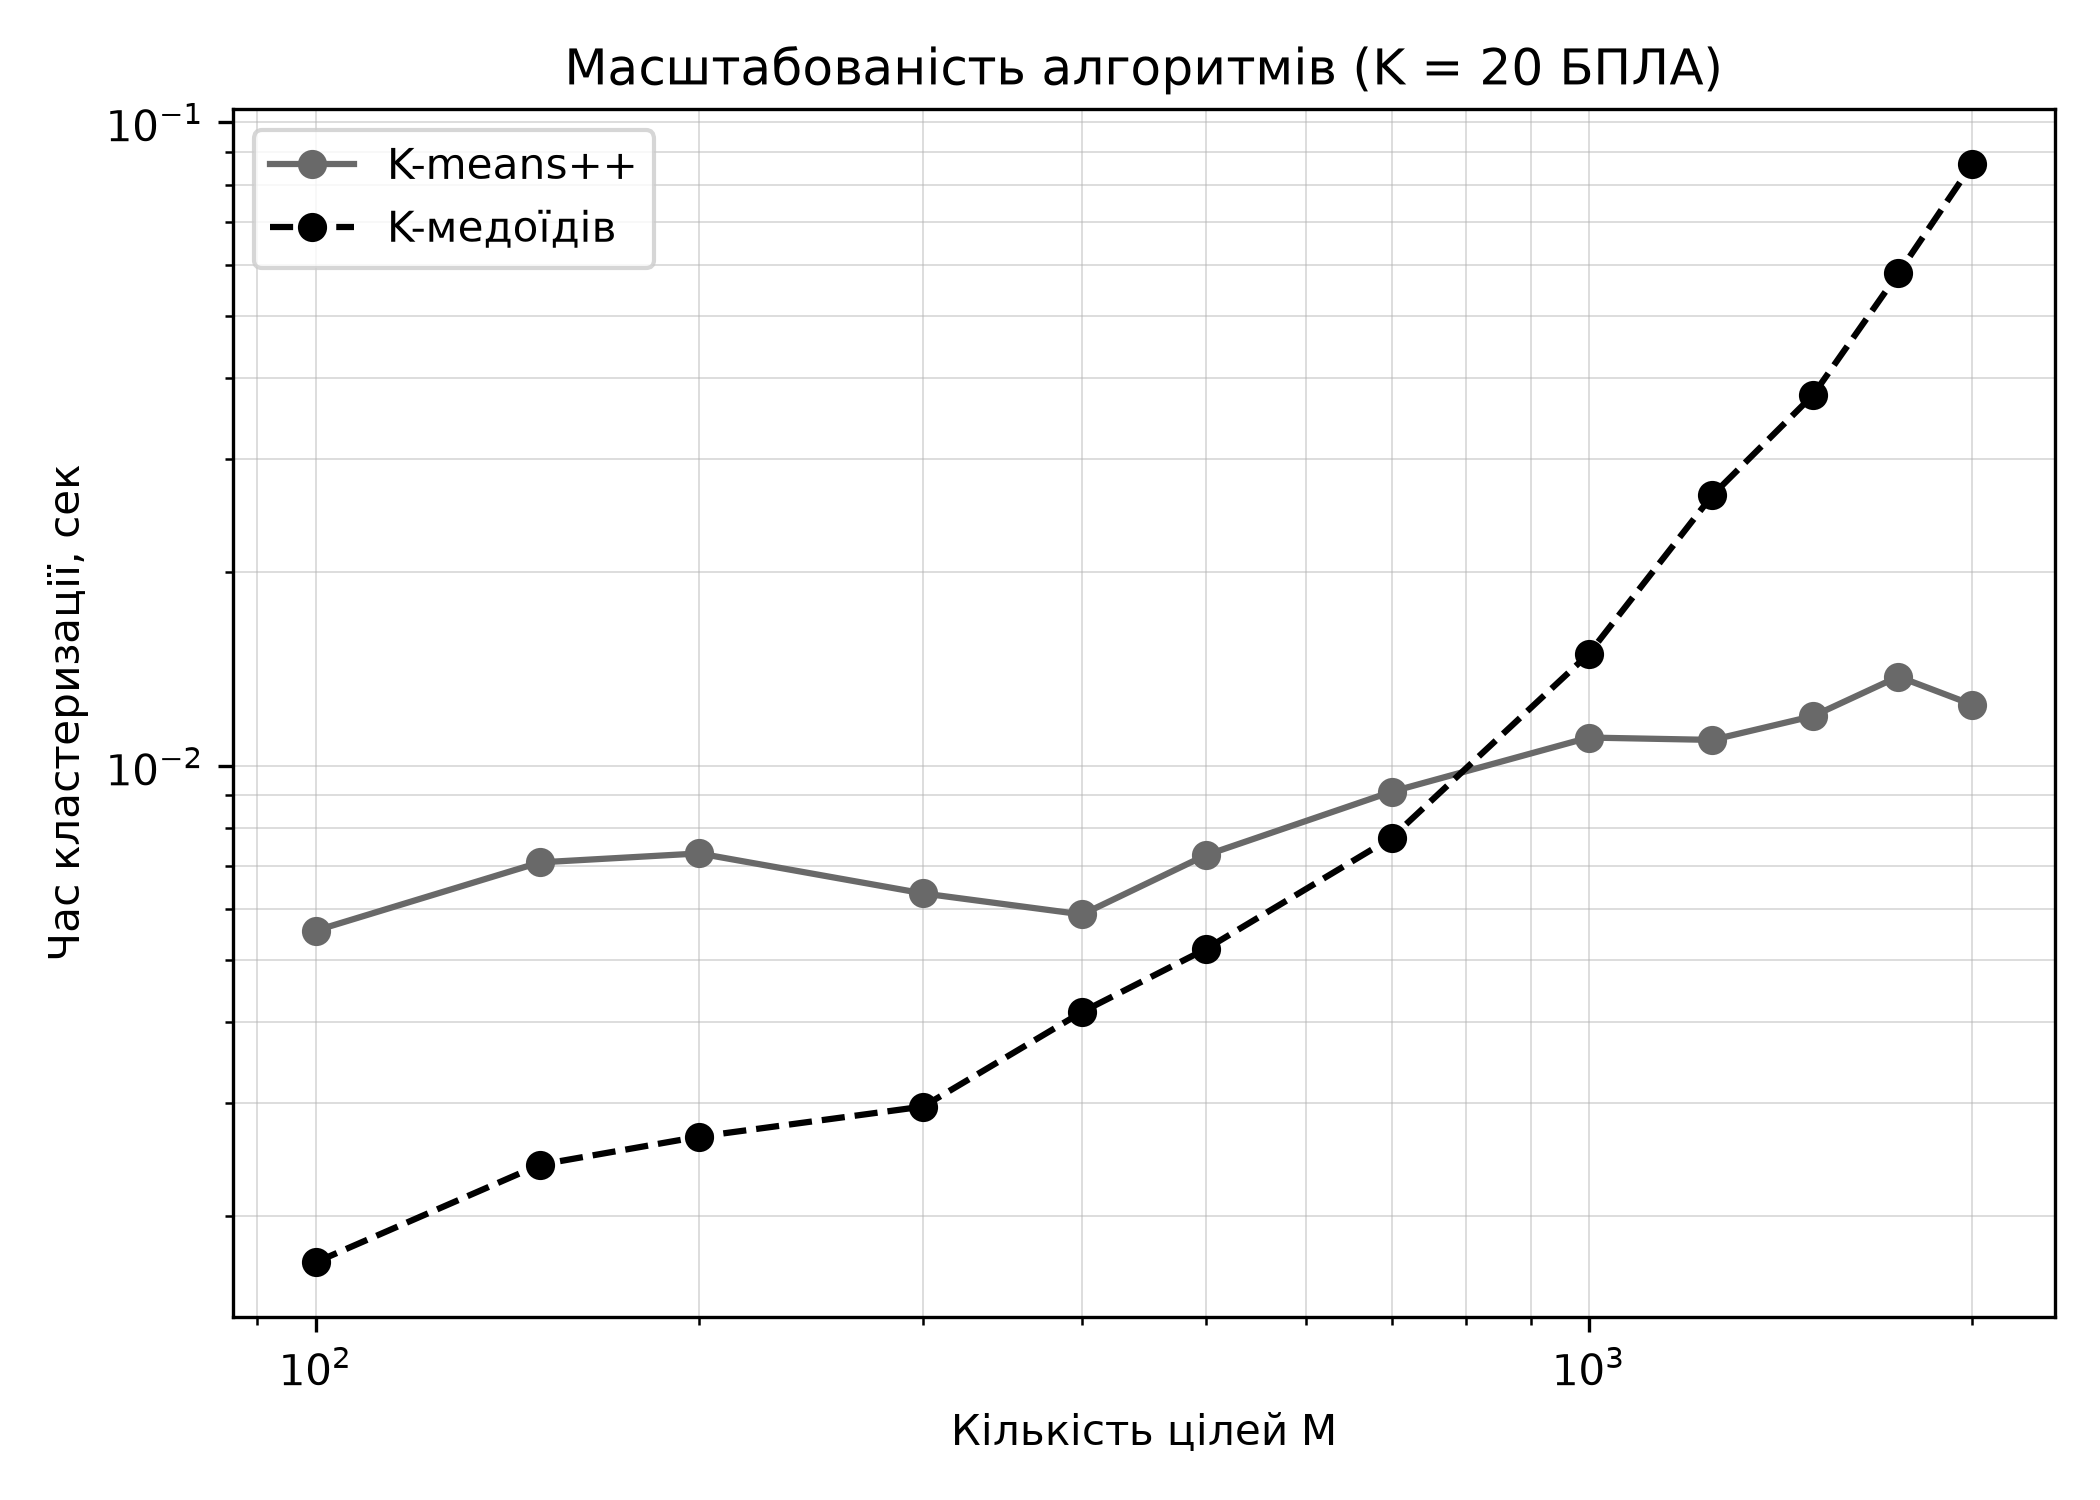
\includegraphics[width=0.85\textwidth,height=0.78\textheight,keepaspectratio]{scalability_K20.png}
    \end{center}
\end{frame}

\begin{frame}{Порівняння з попередніми результатами}
    \heading{Що було у попередній презентації}
    Для $M=2000$, $K=20$ та $1\%$ викидів у попередньому експерименті $K$-медоїдів показував кращі маршрутні показники, ніж $K$-середніх.

    \bigskip
    \heading{Що цікаво в нашому експерименті}
    У нашій реалізації при великих $M$ метод $K$-медоїдів має значно більший час кластеризації, а маршрутні показники відрізняються від попередньої поведінки.

    \bigskip
    \begin{center}
        \bfseries
        Це означає, що потрібно окремо перевірити вплив реалізації K-медоїдів, параметрів генерації сценаріїв і відповідність моделі попередній роботі.
    \end{center}
\end{frame}

% ============================================================
\section{Висновки}

\begin{frame}{Висновки та подальша перевірка}
    \begin{enumerate}
        \item У роботі розглянуто дворівневу схему:
        \[
            \text{кластеризація рухомих цілей}\quad\longrightarrow\quad\text{маршрутизація БПЛА}.
        \]

        \item Для обох методів у головному експерименті забезпечено перехоплення $100\%$ цілей.

        \item Порівнювались не внутрішні цільові функції кластеризації, а кінцеві показники маршрутизації: середній та максимальний час, середня та максимальна довжина.

        \item Отримані відмінності від попередньої роботи вказують на потребу перевірити реалізацію $K$-медоїдів, зокрема порівняти її з PAM/FasterPAM.
    \end{enumerate}
\end{frame}

\begin{frame}{Джерела}
    \footnotesize
    \begin{thebibliography}{9}
        \bibitem{skybytskyi2025slides}
        Н. М. Скибицький.
        \newblock \emph{Алгоритми апроксимації розв'язків робастних задач комбінаторної оптимізації}.
        \newblock Науковий семінар «Теорія оптимальних рішень», 23 грудня 2025.

        \bibitem{skybytskyi2025uav}
        N. M. Skybytskyi.
        \newblock Two-level algorithm for the UAVRP with moving targets.
        \newblock \emph{Cybernetics and Computer Technologies}, 4(4):29--36, 2025.

        \bibitem{arthur2007}
        D. Arthur, S. Vassilvitskii.
        \newblock k-means++: The Advantages of Careful Seeding.
        \newblock SODA, 2007.

        \bibitem{kaufman1990}
        L. Kaufman, P. J. Rousseeuw.
        \newblock \emph{Finding Groups in Data: An Introduction to Cluster Analysis}.
        \newblock Wiley, 1990.
    \end{thebibliography}
\end{frame}

\end{document}
